\section{F3 Netze e.V.}

\begin{frame}{}
    \begin{center}
        F3 Netze e.V.
     \end{center}
\end{frame}

\begin{frame}{Verein ?}
    \begin{columns}[T]
        \begin{column}{0.45\textwidth}
            Was ist F3 Netze e.V.
            \begin{itemize}
                \item Infrastrukturverein
                \item IP-Ressourcen
                \item Provider $\rightarrow$ Traffic ''ausleiten''
                \item Standortüberlassungen
                \item Teilnehmer vom Freifunk Netz
                \item \underline{Keine} Community Vertretung
            \end{itemize}
        \end{column}
        \begin{column}{0.45\textwidth}
            Was tut F3 Netze e.V.
            \begin{itemize}
                \item Freifunk Gateways
                \item Richtfunk-Standorte
                \item Tor Exit
                \item BFWA Frequenzen
            \end{itemize}
        \end{column}
    \end{columns}
\end{frame}

\begin{frame}{Z-Bau}
    \only<1>{
        \begin{itemize}
            \item IP-Ressourcen von den Zwiebelfreunde e.V.
            \begin{itemize}
                \item AS205100
                \item 185.220.100.0/24
                \item 2a0b:f4c0::/32
            \end{itemize}
            \item Glasfaser zum Nürnberg Internet Exchange (N-IX)
            \begin{itemize}
                \item 10 GBit/s Port von 
\includegraphics[height=1em]{img/proact}
                \item 800 MBit/s Transit
                \item $\sim$38 Peerings
            \end{itemize}
            \item[$\rightarrow$] Aktuell ~400 MBit/s Tor Exit Traffic
        \end{itemize}
    }
    \only<2>{
        \center
        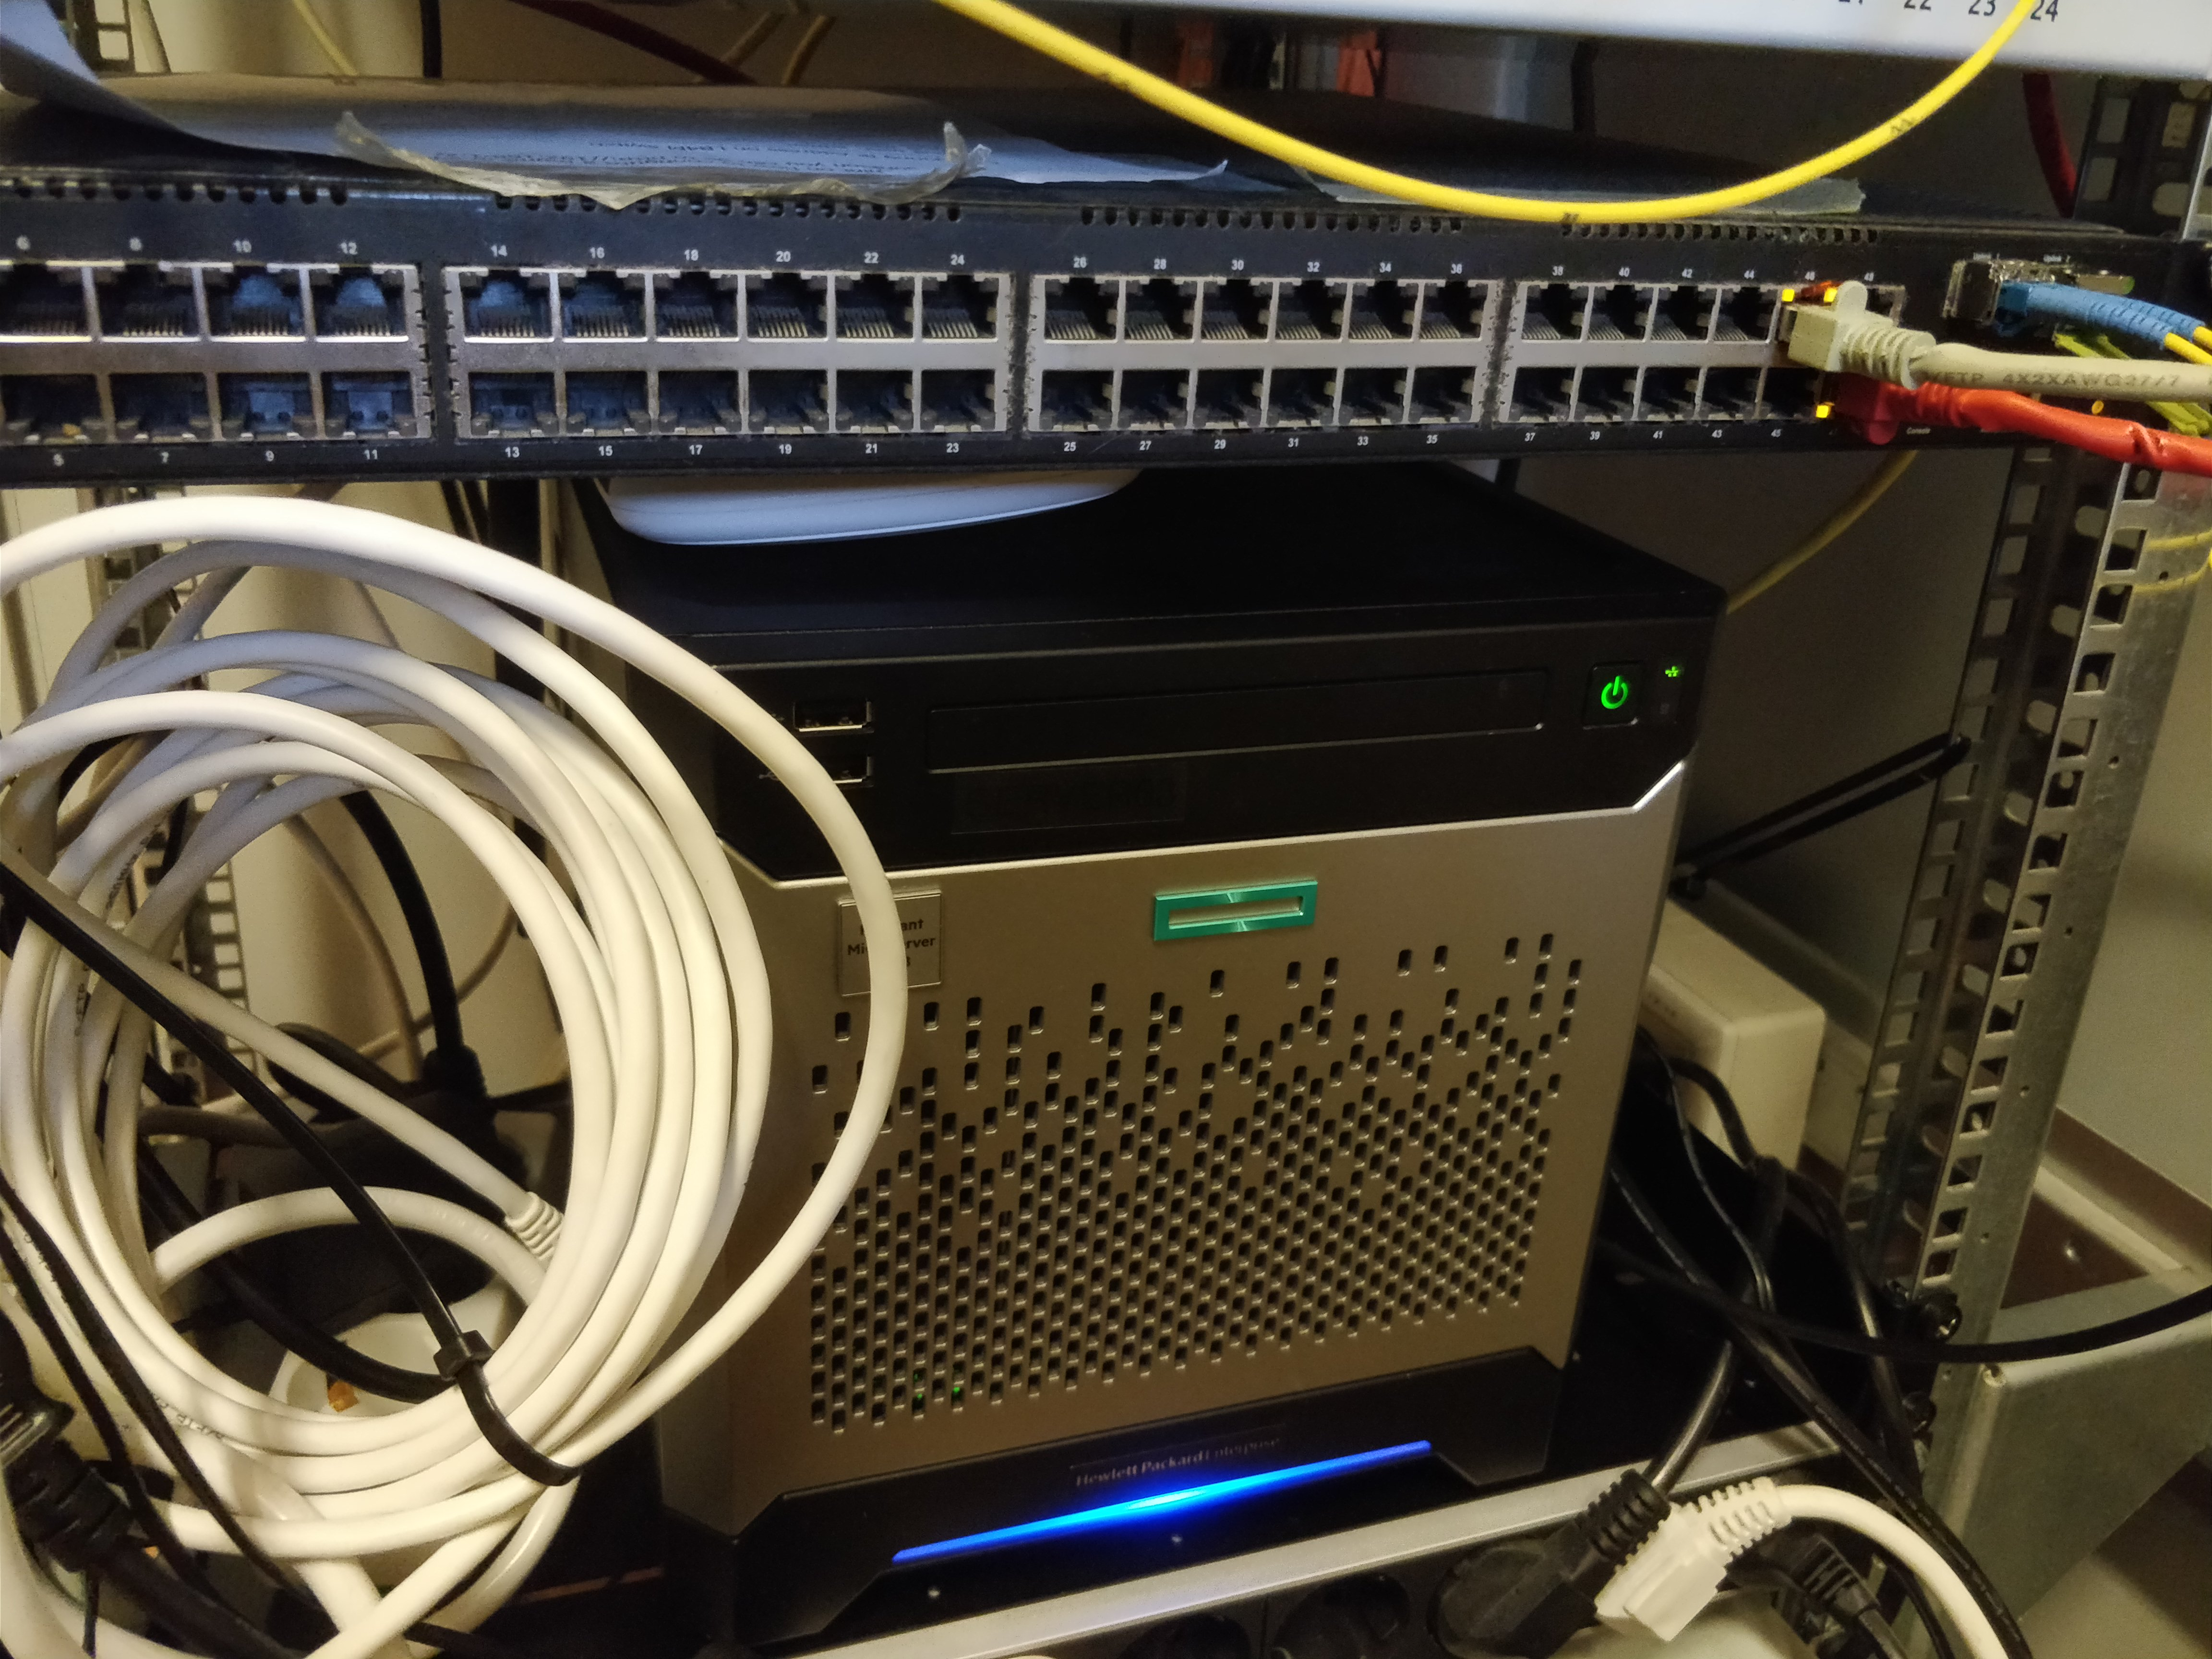
\includegraphics[height=0.86\textheight]{img/zbau-server}
    }
    \only<3>{
        \center
        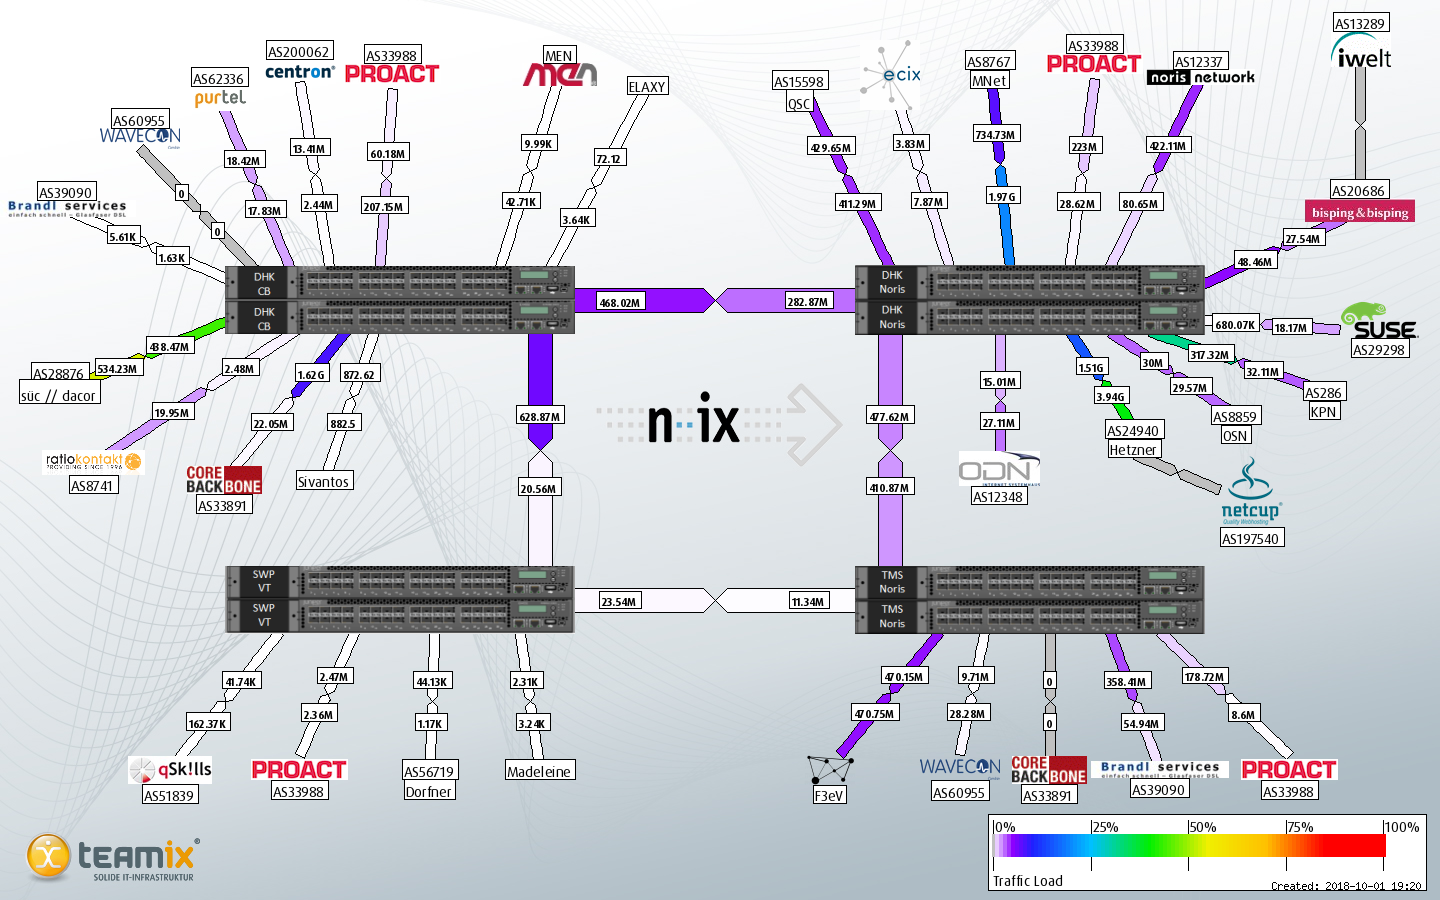
\includegraphics[height=0.86\textheight]{img/NIX}
    }
\end{frame}

\begin{frame}{Gemeinnützigkeit}
    \begin{columns}[T]
        \begin{column}{0.6\textwidth}
            \begin{itemize}
                \item Gemeinnützigkeit noch nicht anerkannt
                \item Verfahren pausiert
                \item AO §52 führt nicht abschließende Liste von Themen
                \item[:(] Laut AEAO Liste abschließend
                \item[:(] Laut AEAO ''Internetvereine'' per se nicht gemeinnützig
            \end{itemize}
        \end{column}
        \begin{column}{0.35\textwidth}
            
\includegraphics[width=\textwidth]{img/betterplace}
        \end{column}
    \end{columns}

    \vfill

    $\rightarrow$ Help needed\\
    \url{https://www.betterplace.org/de/projects/60168}

    \vfill
\end{frame}

